\section{Comparison}
\label{sect:results:comparison}
\begin{itemize}
  \item Ha to-tre eksempelqueries, som bare bruker de operatorene som den LL vi dekket st\o tter, mao: ingen
  pathExprs eller predikat
  \item vise som DAG og som tre
  \item sammenligne reads, writes og computes mellom de forskjellige m\aa tene
  \item bruke unormaliserte versjoner, presisere at de er unormaliserte.. (ikkeno normalisering for oss heller, av
  rettferdighetsgrunner)
  \item Viktig \aa~ f\aa~ med at v\aa r versjon er langt mer egnet for
  parallellisering! Spesielt siden mars-greiene er spredd over flere maskiner
  osv., uten at vi vet saa mye om arkitekturen. Kanskje Oystein vet mer
\end{itemize}

\begin{figure}[!h]
	\centering
	\mbox{
		\subfigure[MonetDB/Pathfinder]{		
			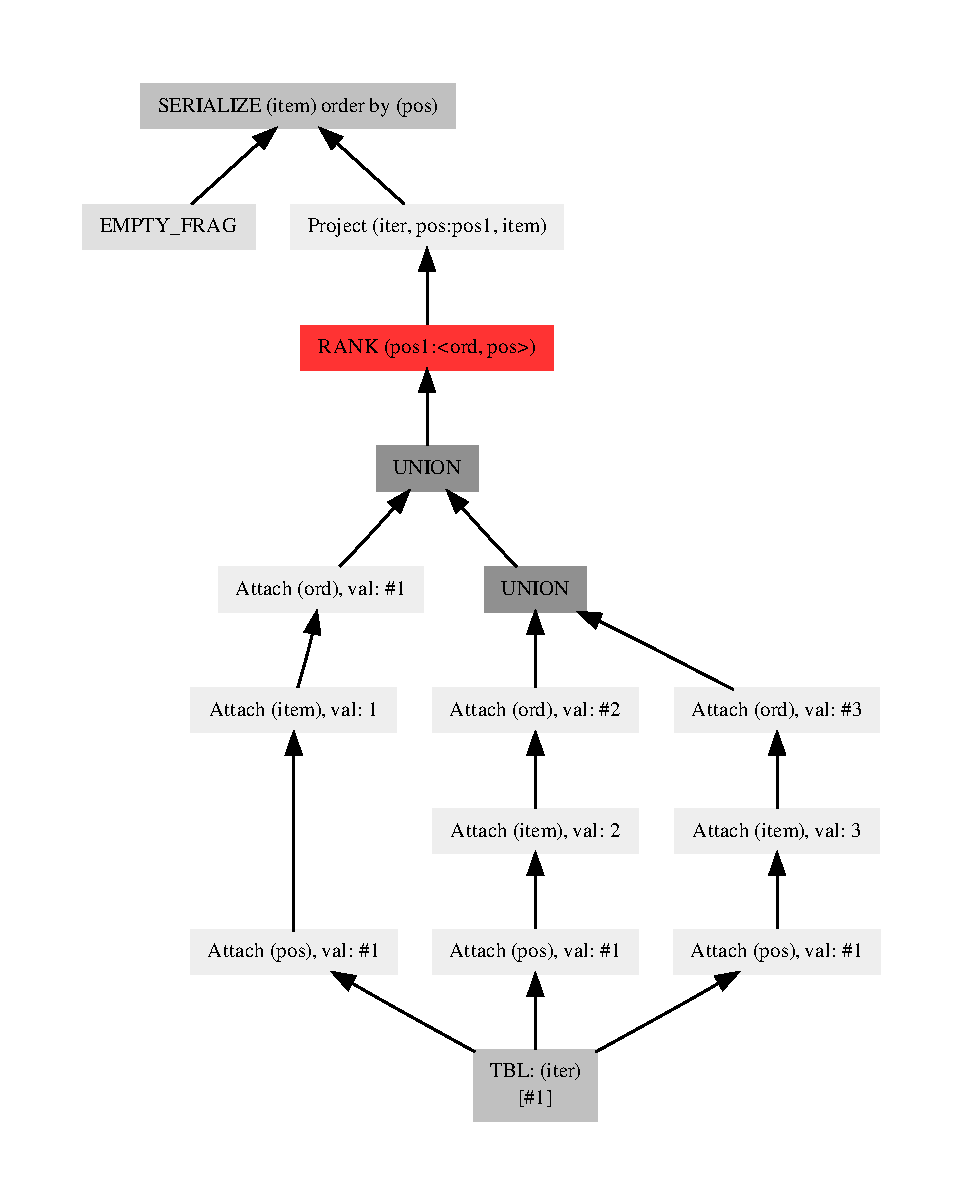
\includegraphics[width=0.5\textwidth]{img/graphs/td_impl_flwor_simple_pathfinder}
			\label{fig:result:comparison:simple_dag}
		}
		\quad
		\subfigure[Prototype implementation]{
		
			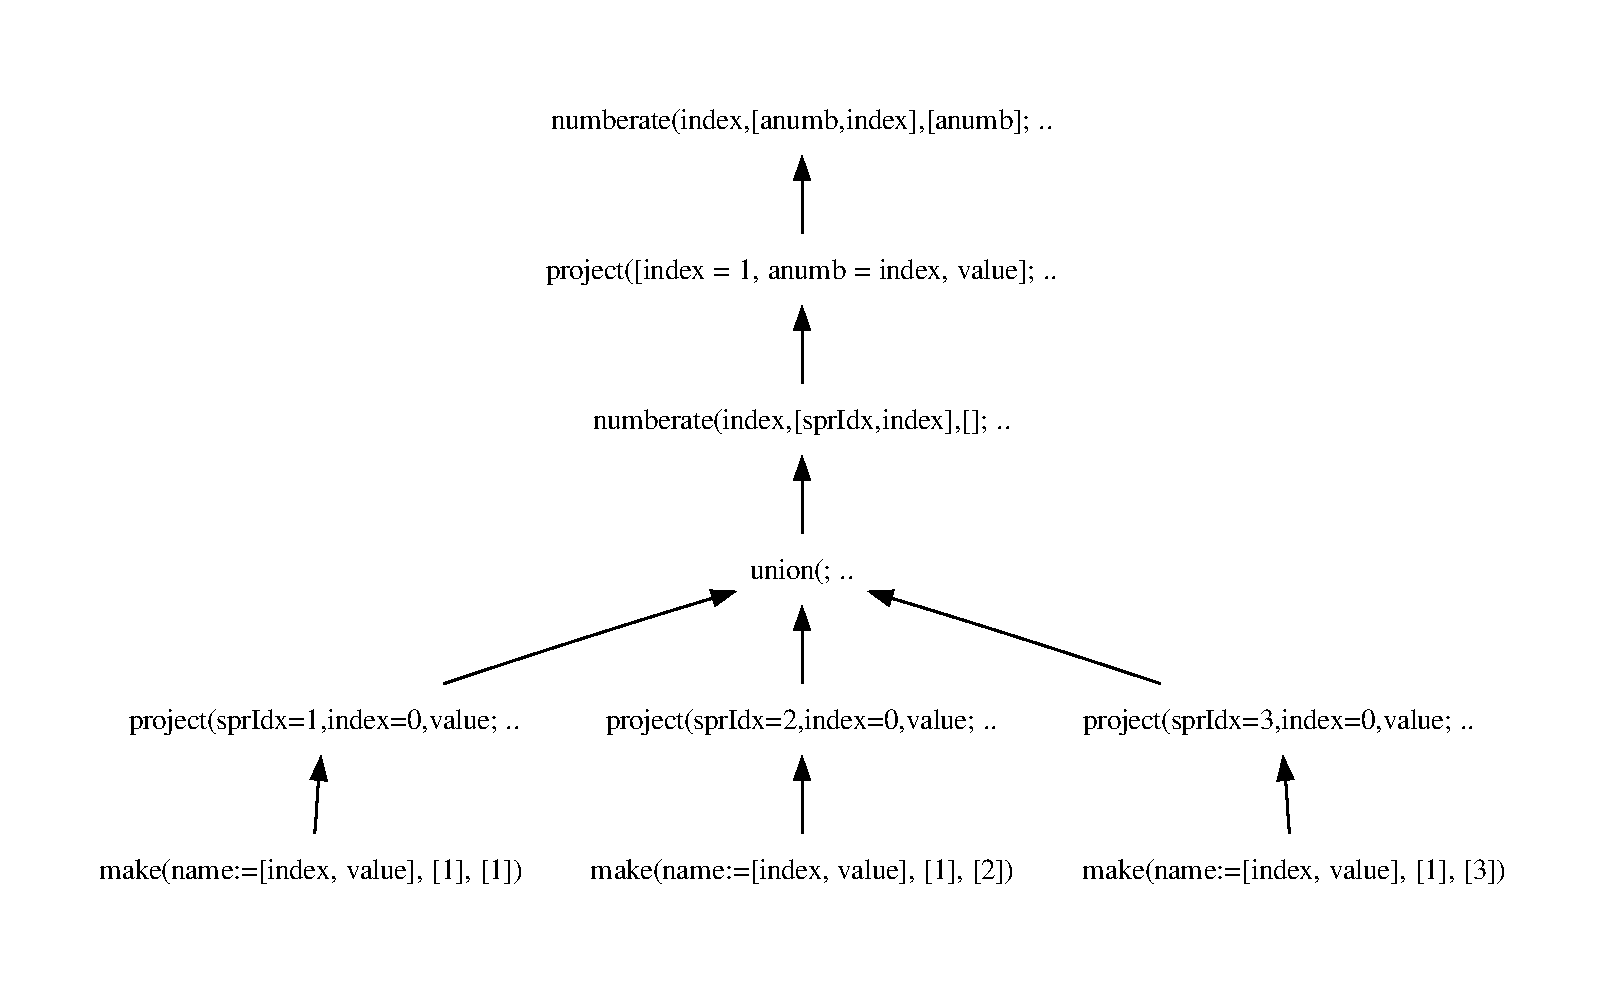
\includegraphics[width=0.5\textwidth]{img/graphs/td_impl_flwor_simple_xq_relalg}
			\label{fig:result:comparison:simple_pathfinder_dag}
		}
	}
	\caption{Comparison of DAGs for the trivial expression in section
	\ref{sect:results:algebra:generated:trivial_flwor}}
\end{figure}

\newpage
\begin{figure}[!h]
	\centering
	\mbox{
		\subfigure[MonetDB/Pathfinder]{		
			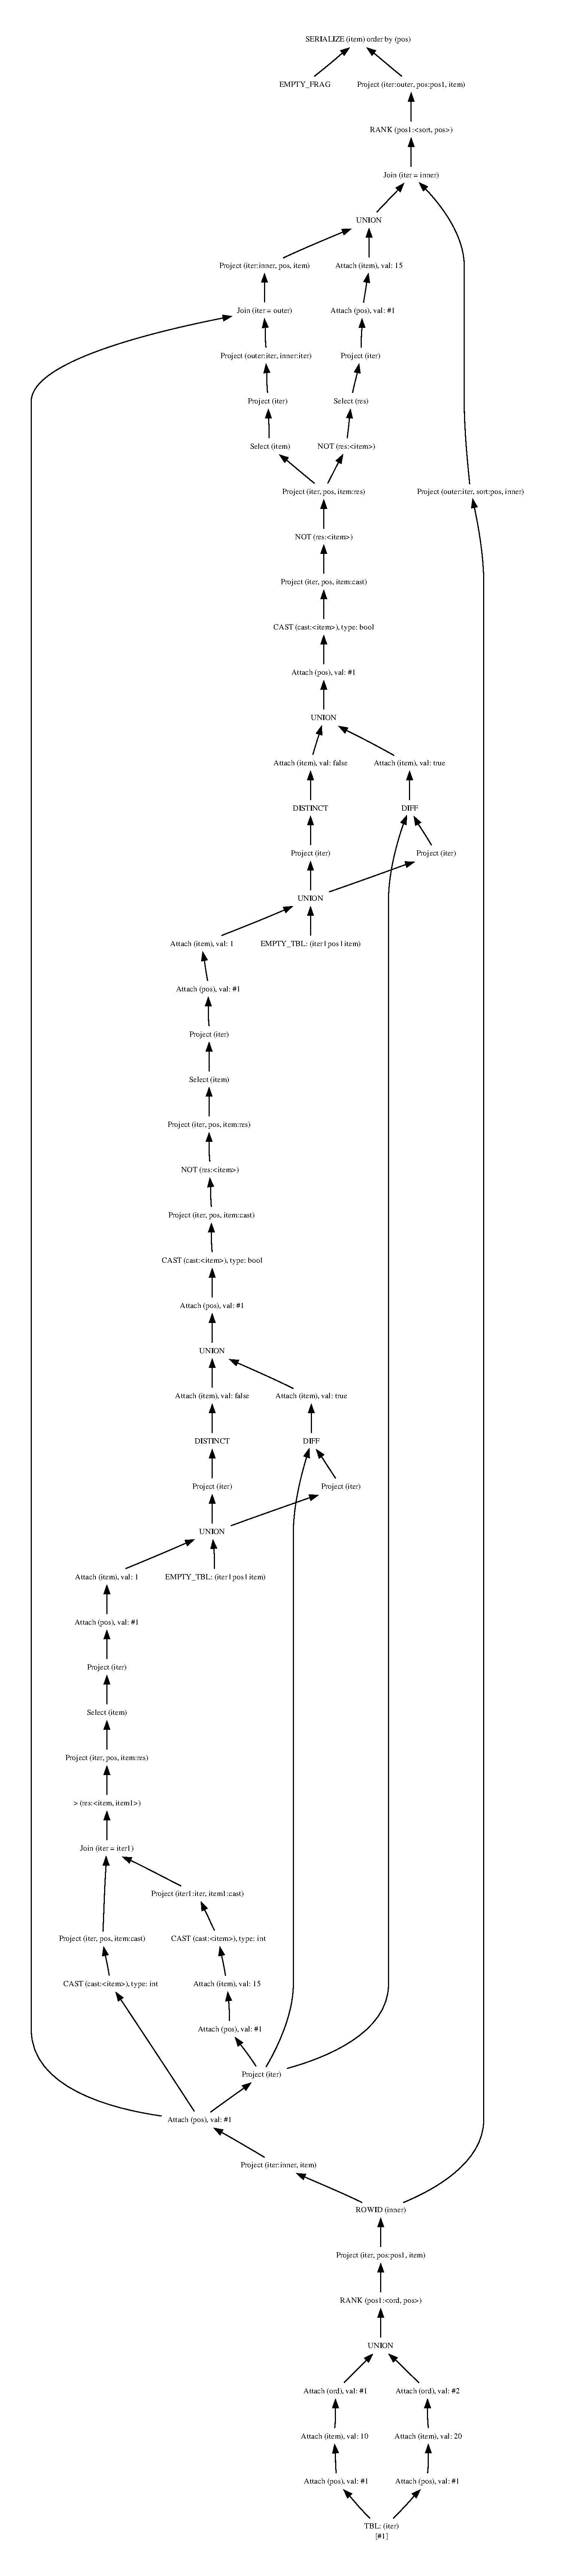
\includegraphics[width=0.3\textwidth]{img/graphs/td_impl_flwor_ifthenelse_pathfinder}
			\label{fig:result:comparison:conditional_dag}
		}
		\quad
		\subfigure[Prototype implementation]{
		
			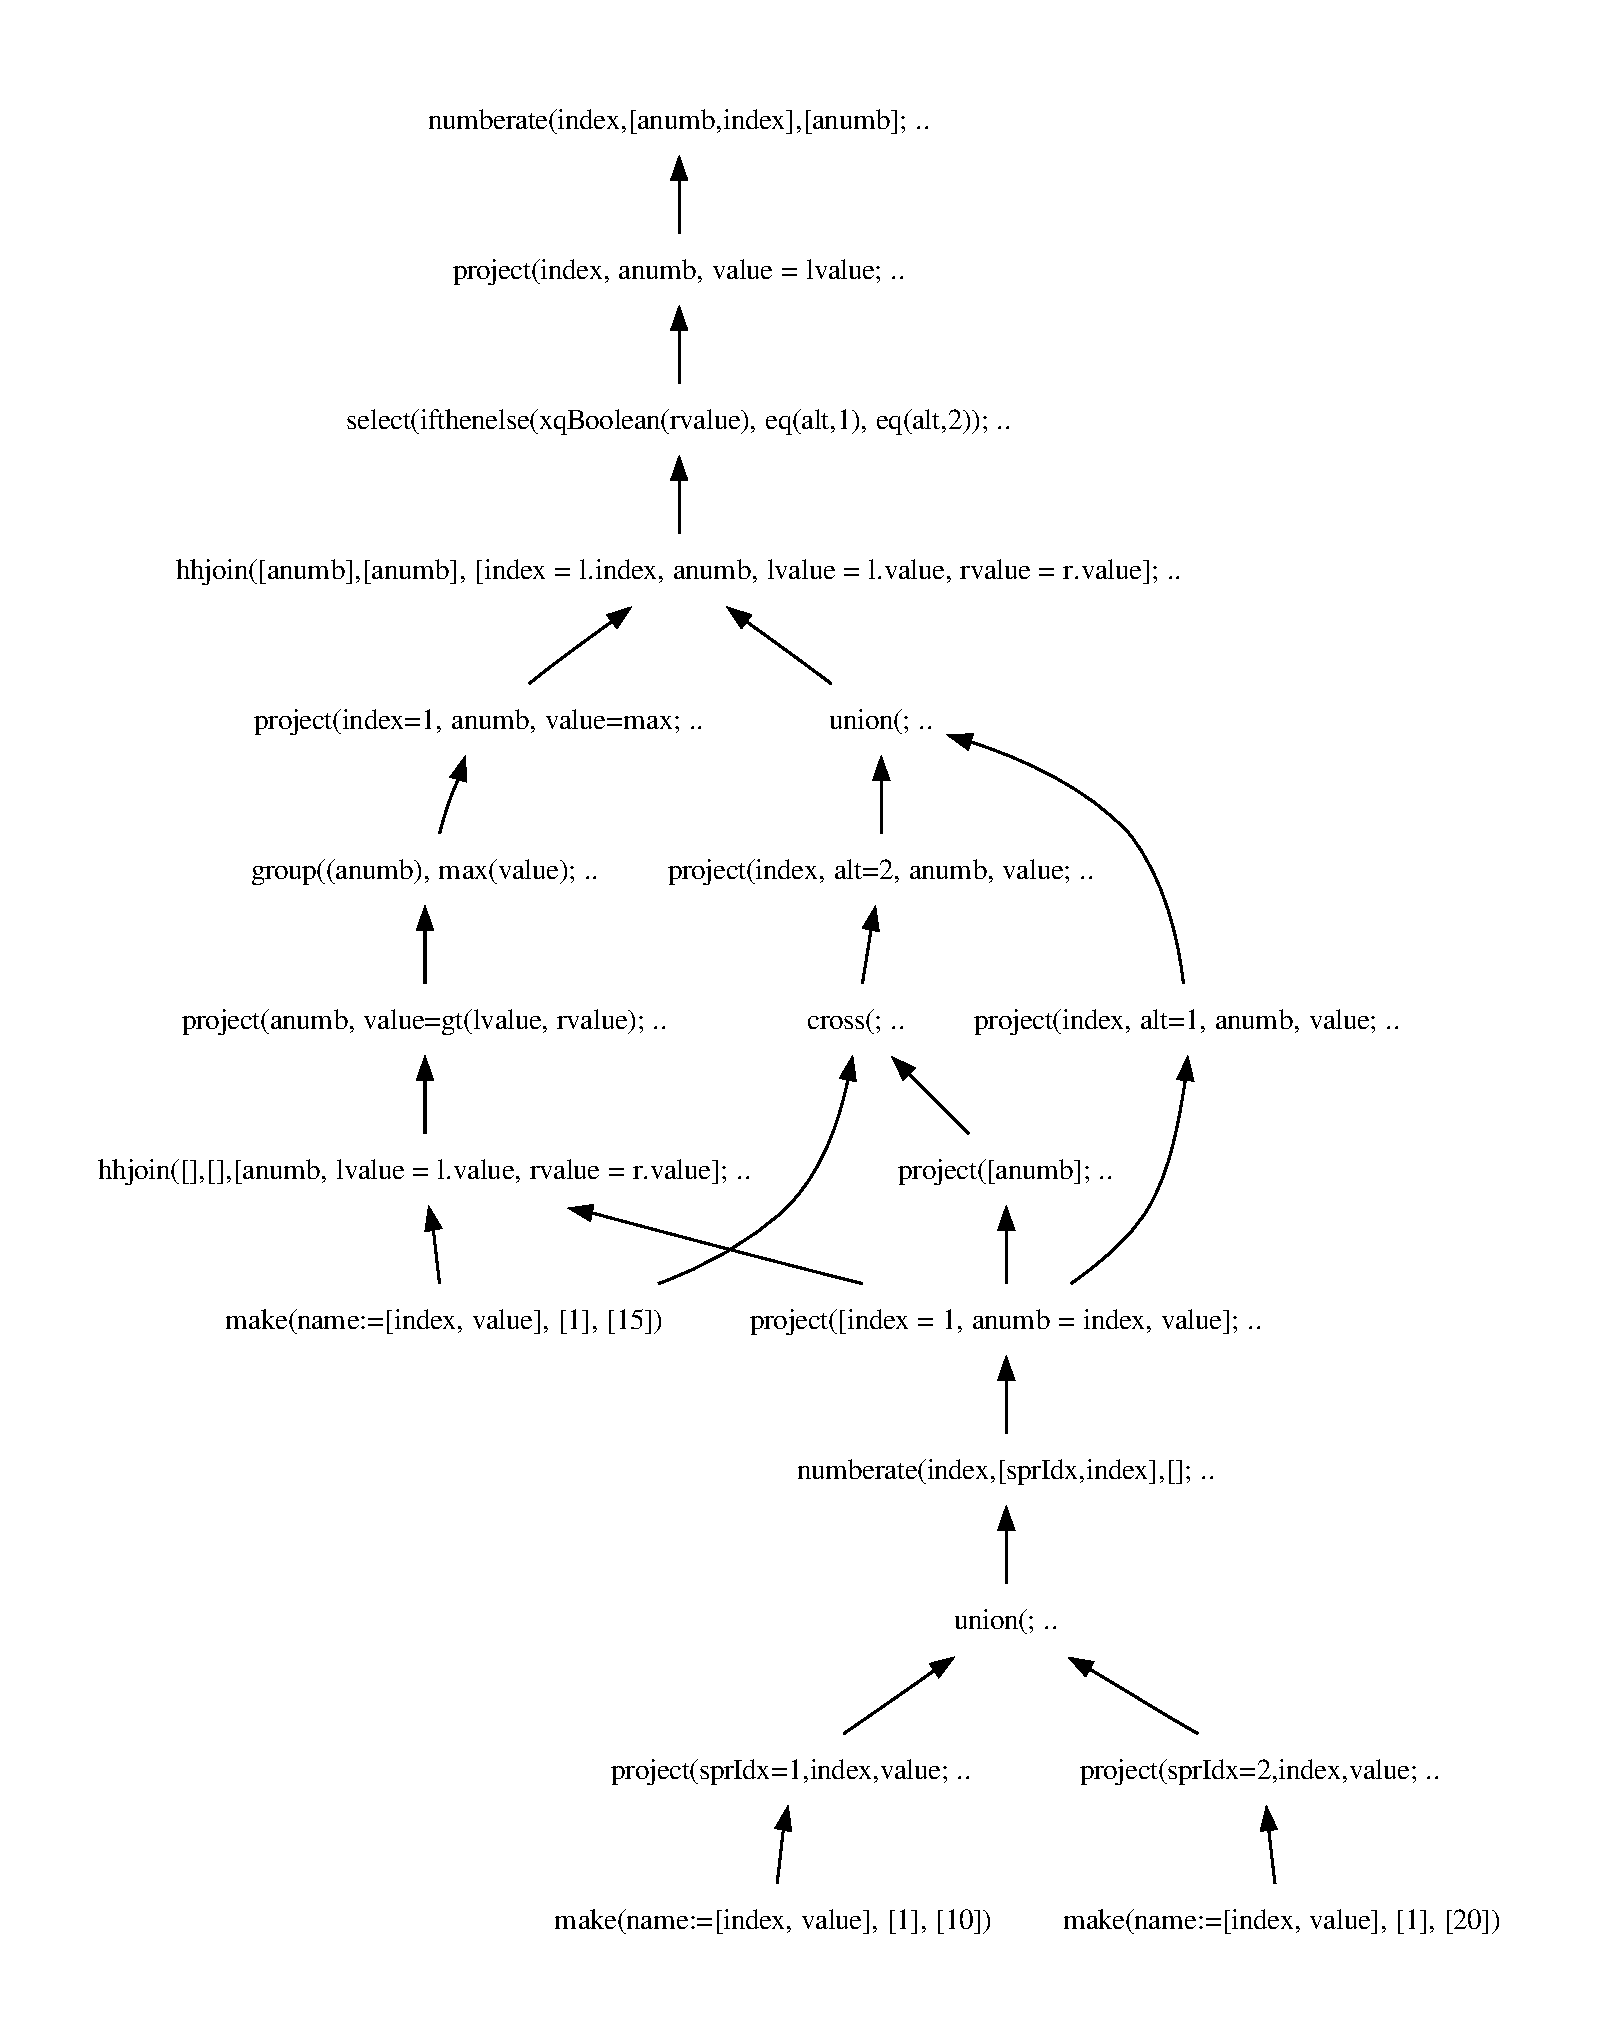
\includegraphics[width=0.7\textwidth]{img/graphs/td_impl_flwor_ifthenelse_xq_relalg_dag}
			\label{fig:result:comparison:conditional_pathfinder_dag}
		}
	}
	\caption{Comparison of DAGs for the conditional expression in section
	\ref{sect:results:algebra:generated:conditional_flwor}}
\end{figure}

\newpage
\begin{figure}[!h]
	\centering
	\mbox{
		\subfigure[MonetDB/Pathfinder]{		
			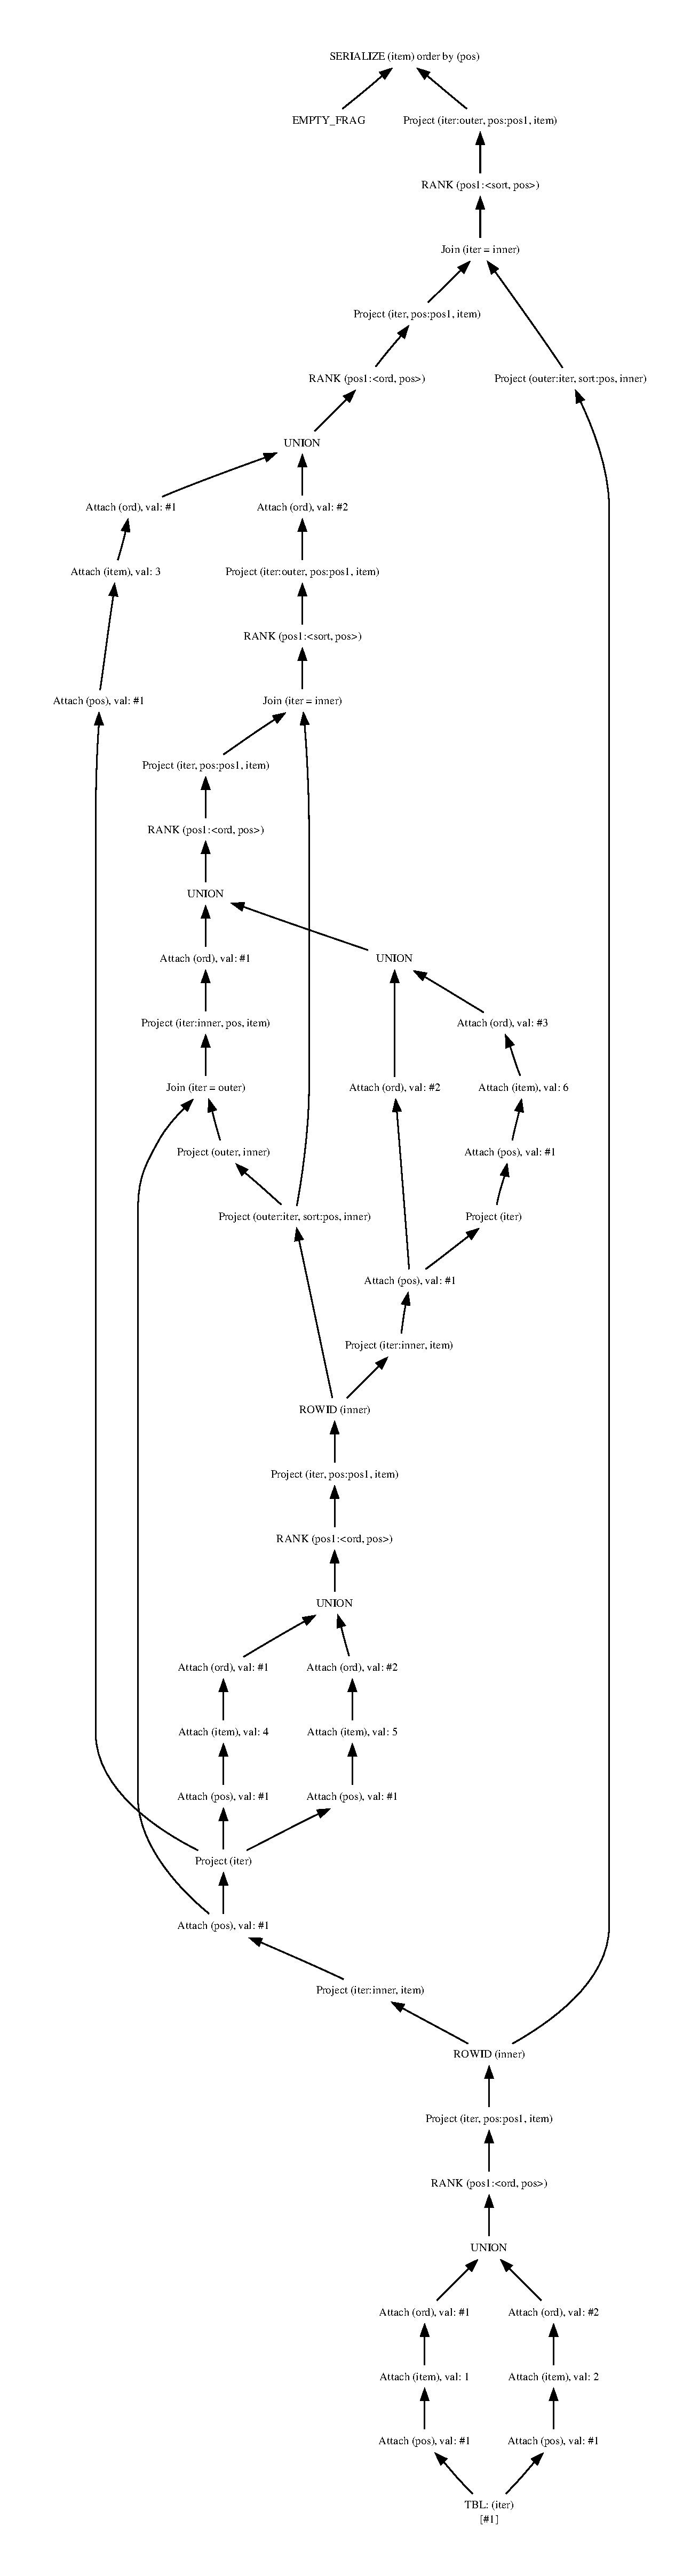
\includegraphics[width=0.37\textwidth]{img/graphs/td_impl_flwor_complex_pathfinder}
			\label{fig:result:comparison:complex_xqft_dag}
		}
		\quad
		\subfigure[Prototype implementation]{
		
			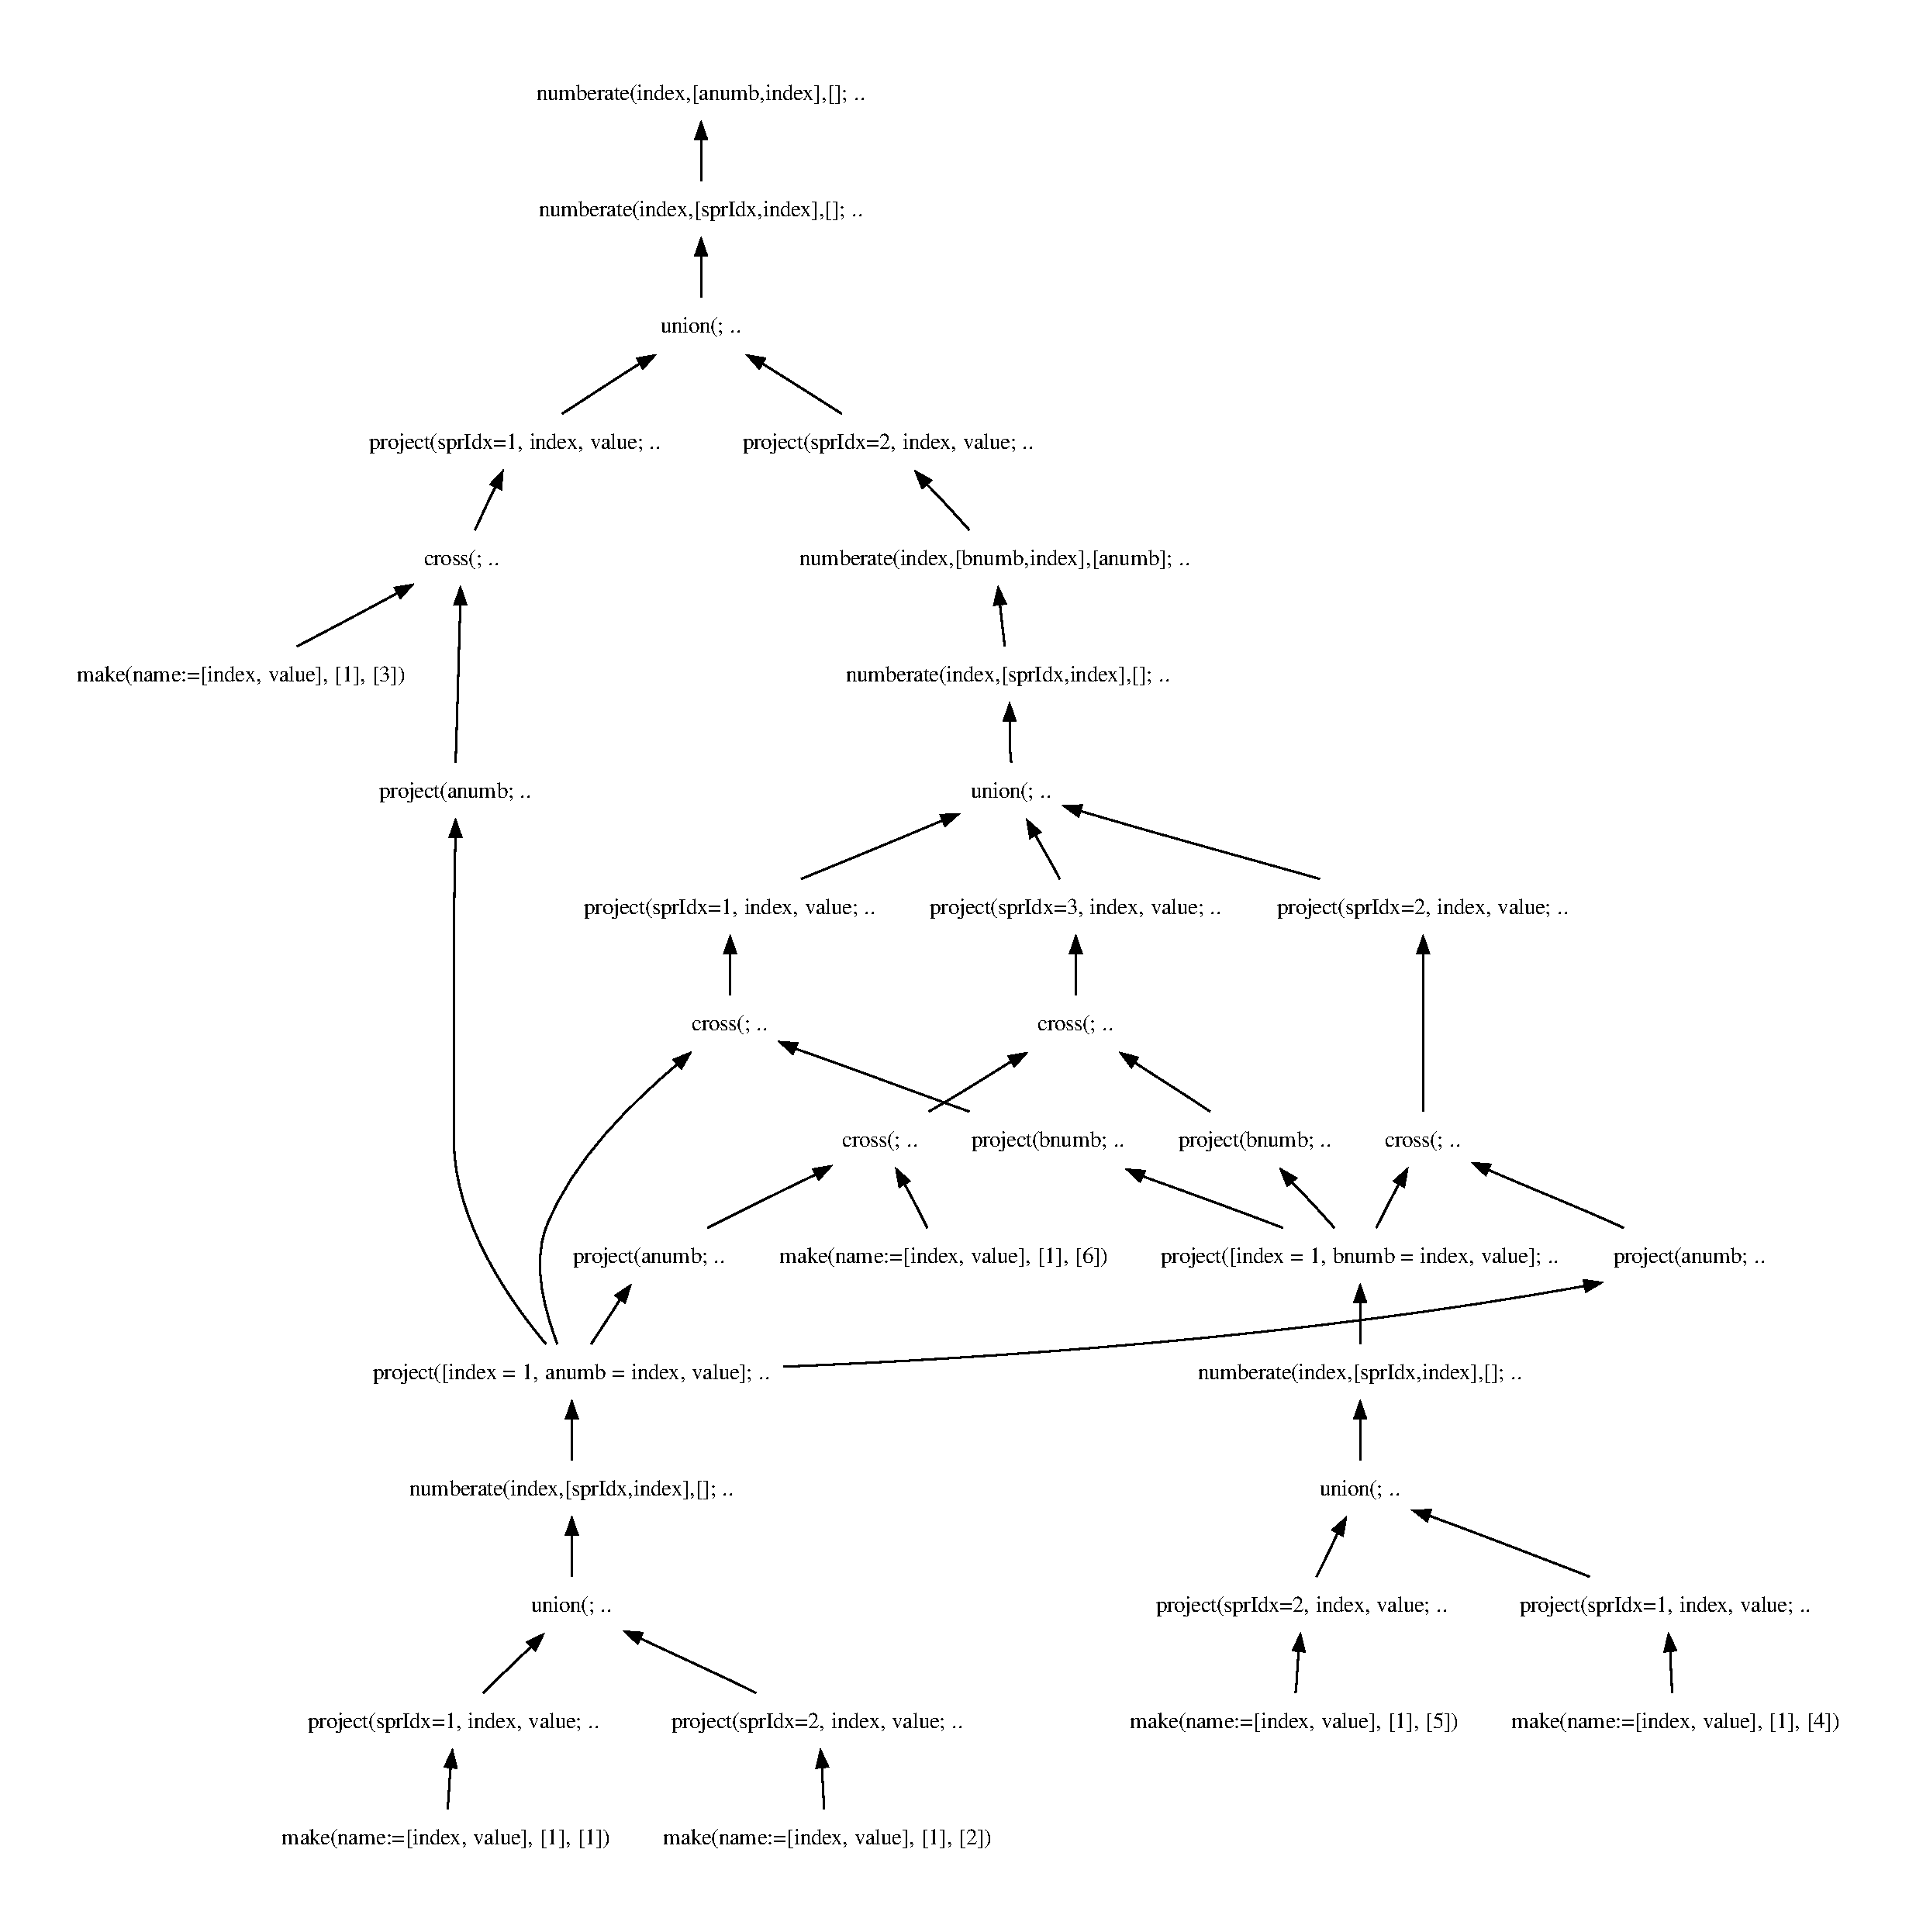
\includegraphics[width=0.6\textwidth]{img/graphs/td_impl_flwor_complex_xq_relalg_dag}
			\label{fig:result:comparison:complex_pathfinder_dag}
		}
	}
	\caption{Comparison of DAGs for the complex expression in section
	\ref{sect:results:algebra:generated:complex_flwor}}
\end{figure}